\section{Eksempel på 'Idea Maturation'}
I dette afsnit vil et eksempel på såkaldt `Idea Maturation' fra \citet[Kapitel 23]{art:essence}.
Specifikt bruger vi en gammel og en ny konfigurationstabel for det implementerede system, og vi undersøger forskellen mellem de to konfigurationer.
Dog er der så mange ændringer, idet den gamle konfigurationstabel blev dannet da systemet var nyt. 
Derfor dækkes kun de mest interessante ændringer i konfigurationstabellen.

De to konfigurationstabeller, kan ses i \cref{tab:tidligKonfigurationsTabel} og \cref{tab:konfigurationsTabel}, henholdsvis den gamle og den nye. 
I den gamle konfigurationstabel er det blevet markeret hvad der er ændret.
I dette vælger vi kun at undersøge ``Evaluation", "Stakeholders" og "Features''. 

Som man kan se i Evaluation, er Procedure blevet ændret fra "fokusgrupper'' til "Fokusgruppemøde, Integrationstest'' og Criteria er blevet ændret fra "Mortens dogmeregler" til at systemet skal være "Modulært, Fleksibelt, Kombinerbar, og Kommunikativ''. \stefan{uddybes?}

I "Stakeholders" er de aktuelle stakeholders blevet ændret fra en masse personer til kun at dække "Sponsorer og Patienter", hvor Patienter ses som main perspective og sponsorer er meget mindre vigtige. 
Grunden til at det blev ændret til dette, var at det var ikke helt klart at patienter var de allervigtigste idet de blev tabt i en liste af forskellige personer.
Ydermere blev Main perspective også specificeret.
Før stod der "Patienter med bipolar affektiv lidelse" hvilket blev ændret til "Patienter med unipolar og bipolar affektive lidelse". 

I "Features", stod der før f.eks. "Stemningslejemeter" og "Stemningsleje dagbog", hvilket ikke passede ind i vision om en objektiv dagbog så derfor blev disse ændret til "Valg og tilpasning af moduler" så patienten selv har kontrol over hvad der overvåges og hvad han kan få information over. Derudover var det stadigvæk vigtigt at patienten kunne visualisere sine data og se på trends, og derfor blev denne beholdt. 

\begin{figure}
	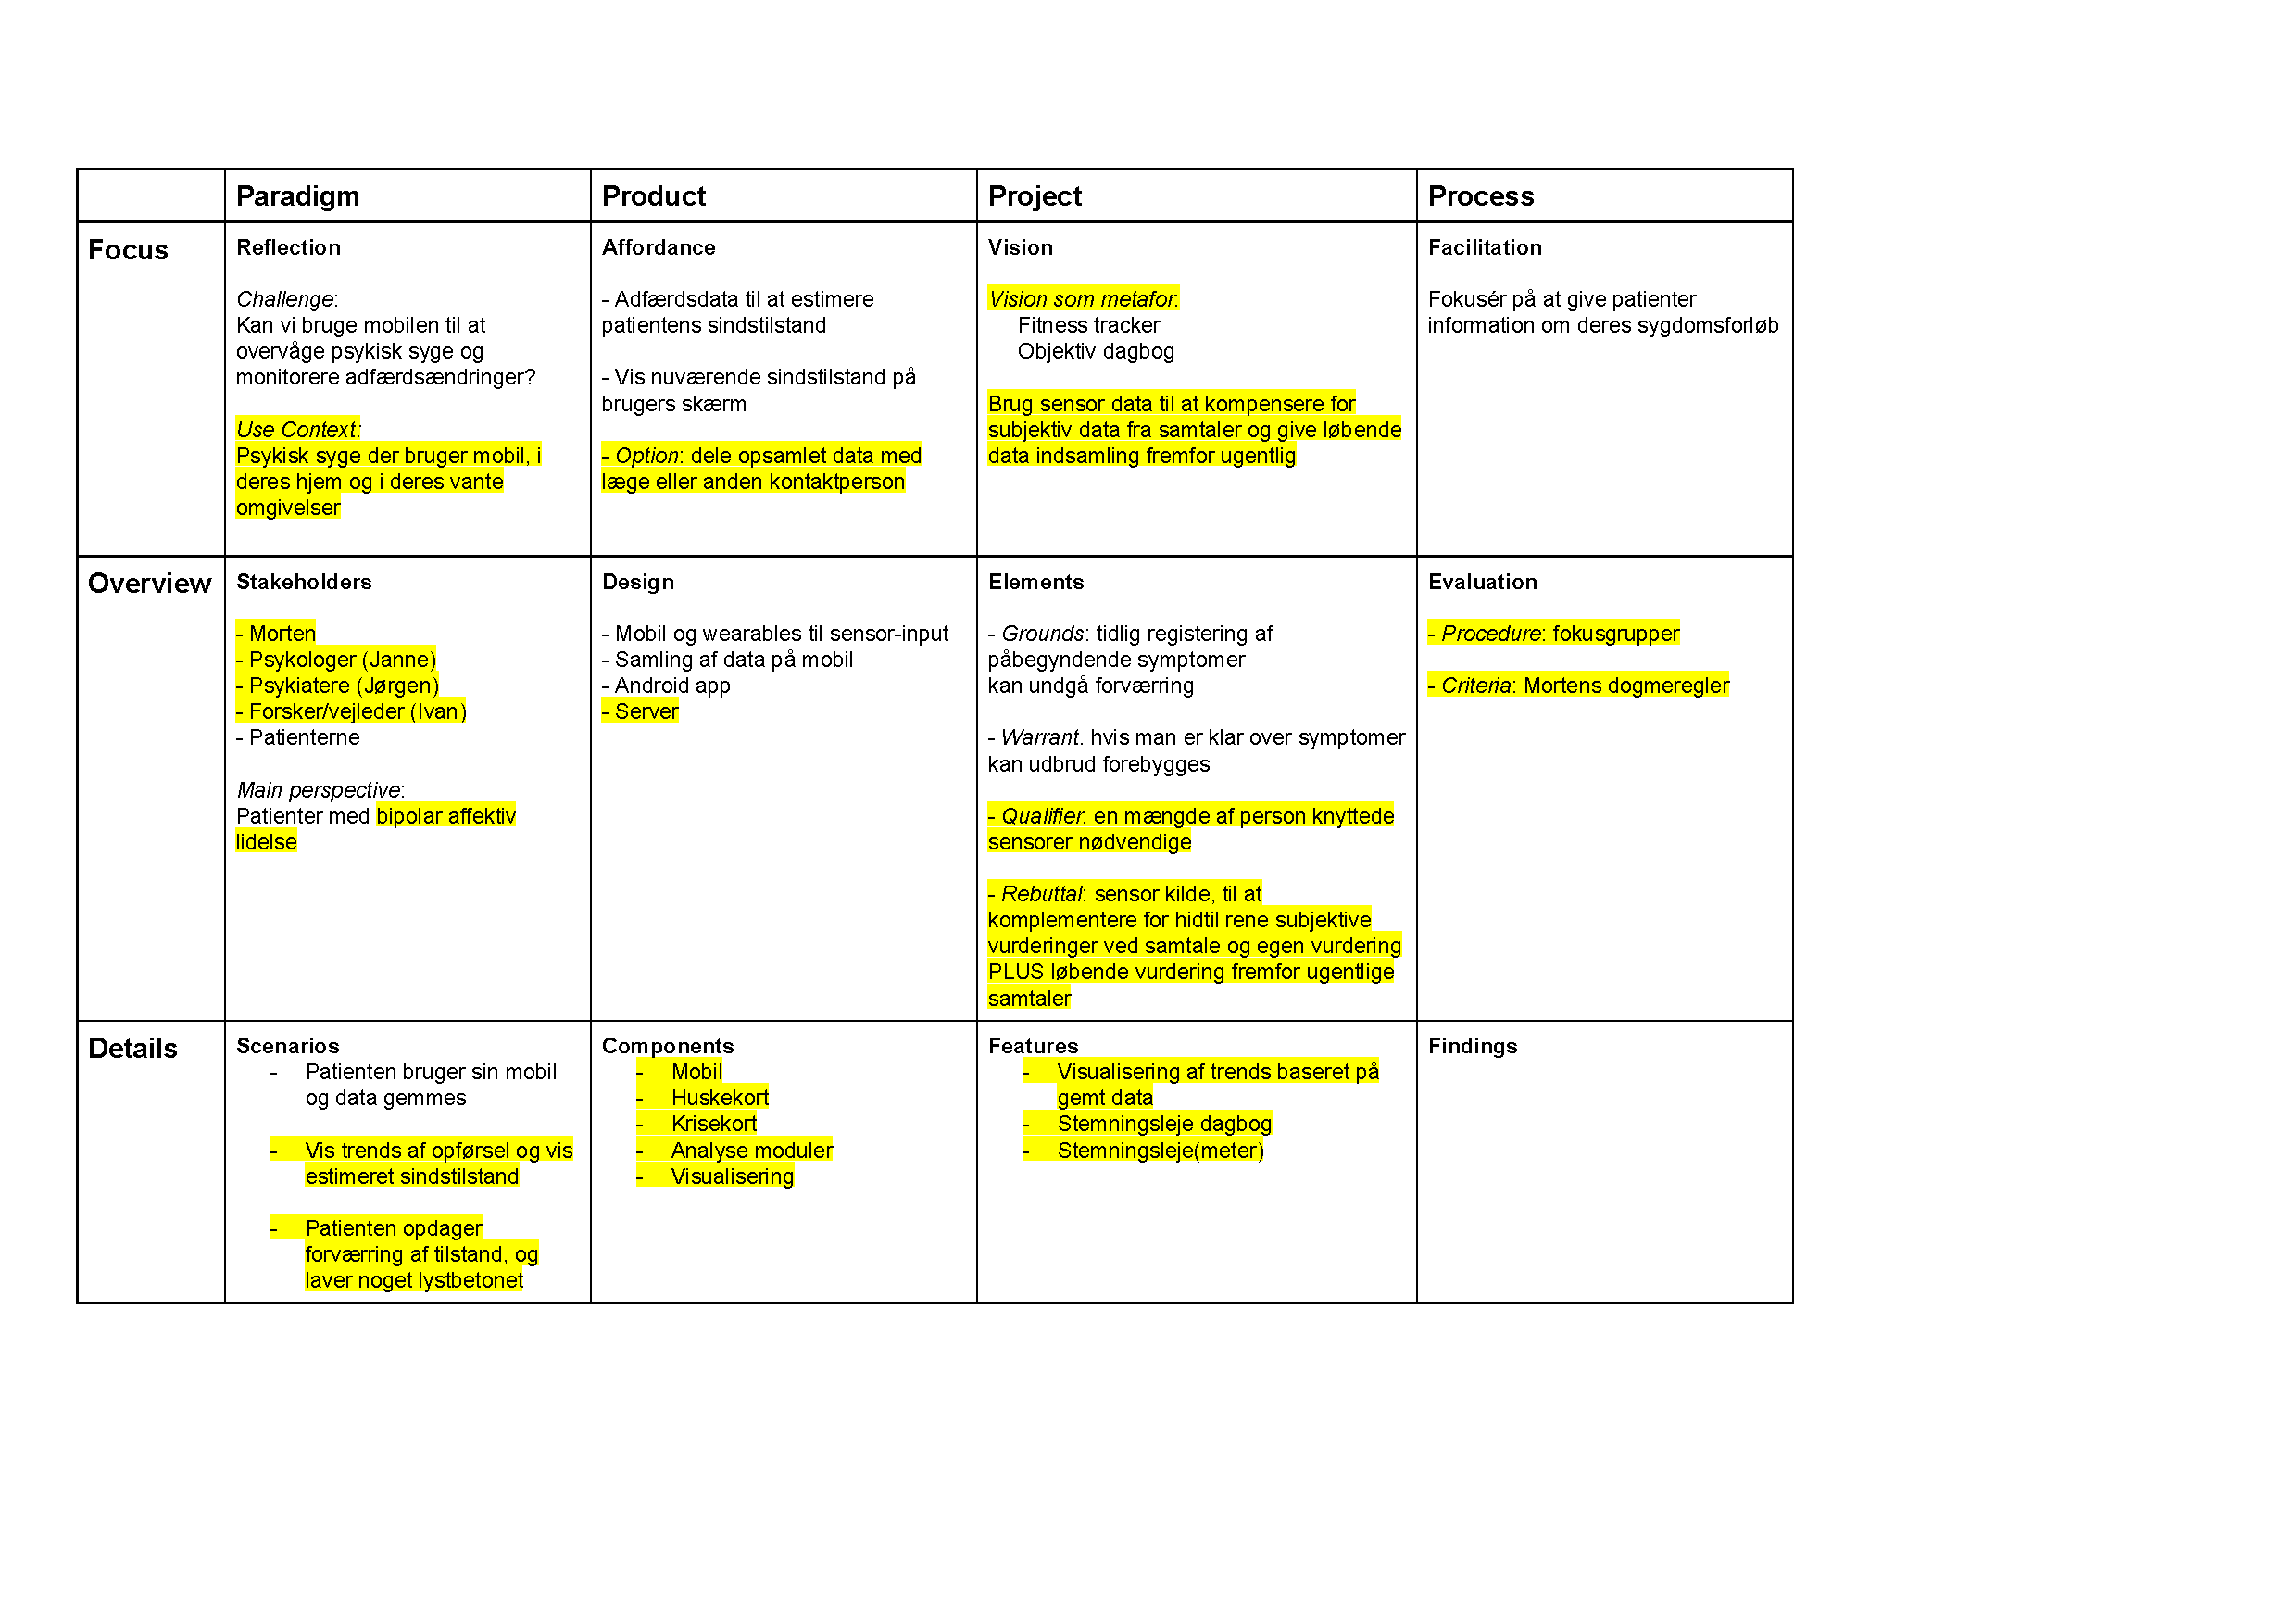
\includegraphics[scale = 0.65,trim = 1cm 3cm 6cm 2cm, angle = 90, clip]{tidlig-konfigurationstabel.pdf}
	\caption{En konfigurationstabel på et tidligt stadie af udviklingen}
	\label{tab:tidligKonfigurationsTabel}
\end{figure}